\documentclass[twoside]{book}

% Packages required by doxygen
\usepackage{fixltx2e}
\usepackage{calc}
\usepackage{doxygen}
\usepackage[export]{adjustbox} % also loads graphicx
\usepackage{graphicx}
\usepackage[utf8]{inputenc}
\usepackage{makeidx}
\usepackage{multicol}
\usepackage{multirow}
\PassOptionsToPackage{warn}{textcomp}
\usepackage{textcomp}
\usepackage[nointegrals]{wasysym}
\usepackage[table]{xcolor}

% Font selection
\usepackage[T1]{fontenc}
\usepackage[scaled=.90]{helvet}
\usepackage{courier}
\usepackage{amssymb}
\usepackage{sectsty}
\renewcommand{\familydefault}{\sfdefault}
\allsectionsfont{%
  \fontseries{bc}\selectfont%
  \color{darkgray}%
}
\renewcommand{\DoxyLabelFont}{%
  \fontseries{bc}\selectfont%
  \color{darkgray}%
}
\newcommand{\+}{\discretionary{\mbox{\scriptsize$\hookleftarrow$}}{}{}}

% Page & text layout
\usepackage{geometry}
\geometry{%
  a4paper,%
  top=2.5cm,%
  bottom=2.5cm,%
  left=2.5cm,%
  right=2.5cm%
}
\tolerance=750
\hfuzz=15pt
\hbadness=750
\setlength{\emergencystretch}{15pt}
\setlength{\parindent}{0cm}
\setlength{\parskip}{3ex plus 2ex minus 2ex}
\makeatletter
\renewcommand{\paragraph}{%
  \@startsection{paragraph}{4}{0ex}{-1.0ex}{1.0ex}{%
    \normalfont\normalsize\bfseries\SS@parafont%
  }%
}
\renewcommand{\subparagraph}{%
  \@startsection{subparagraph}{5}{0ex}{-1.0ex}{1.0ex}{%
    \normalfont\normalsize\bfseries\SS@subparafont%
  }%
}
\makeatother

% Headers & footers
\usepackage{fancyhdr}
\pagestyle{fancyplain}
\fancyhead[LE]{\fancyplain{}{\bfseries\thepage}}
\fancyhead[CE]{\fancyplain{}{}}
\fancyhead[RE]{\fancyplain{}{\bfseries\leftmark}}
\fancyhead[LO]{\fancyplain{}{\bfseries\rightmark}}
\fancyhead[CO]{\fancyplain{}{}}
\fancyhead[RO]{\fancyplain{}{\bfseries\thepage}}
\fancyfoot[LE]{\fancyplain{}{}}
\fancyfoot[CE]{\fancyplain{}{}}
\fancyfoot[RE]{\fancyplain{}{\bfseries\scriptsize Generated by Doxygen }}
\fancyfoot[LO]{\fancyplain{}{\bfseries\scriptsize Generated by Doxygen }}
\fancyfoot[CO]{\fancyplain{}{}}
\fancyfoot[RO]{\fancyplain{}{}}
\renewcommand{\footrulewidth}{0.4pt}
\renewcommand{\chaptermark}[1]{%
  \markboth{#1}{}%
}
\renewcommand{\sectionmark}[1]{%
  \markright{\thesection\ #1}%
}

% Indices & bibliography
\usepackage{natbib}
\usepackage[titles]{tocloft}
\setcounter{tocdepth}{3}
\setcounter{secnumdepth}{5}
\makeindex

% Hyperlinks (required, but should be loaded last)
\usepackage{ifpdf}
\ifpdf
  \usepackage[pdftex,pagebackref=true]{hyperref}
\else
  \usepackage[ps2pdf,pagebackref=true]{hyperref}
\fi
\hypersetup{%
  colorlinks=true,%
  linkcolor=blue,%
  citecolor=blue,%
  unicode%
}

% Custom commands
\newcommand{\clearemptydoublepage}{%
  \newpage{\pagestyle{empty}\cleardoublepage}%
}

\usepackage{caption}
\captionsetup{labelsep=space,justification=centering,font={bf},singlelinecheck=off,skip=4pt,position=top}

%===== C O N T E N T S =====

\begin{document}

% Titlepage & ToC
\hypersetup{pageanchor=false,
             bookmarksnumbered=true,
             pdfencoding=unicode
            }
\pagenumbering{alph}
\begin{titlepage}
\vspace*{7cm}
\begin{center}%
{\Large Elba }\\
\vspace*{1cm}
{\large Generated by Doxygen 1.8.14}\\
\end{center}
\end{titlepage}
\clearemptydoublepage
\pagenumbering{roman}
\tableofcontents
\clearemptydoublepage
\pagenumbering{arabic}
\hypersetup{pageanchor=true}

%--- Begin generated contents ---
\chapter{Hierarchical Index}
\section{Class Hierarchy}
This inheritance list is sorted roughly, but not completely, alphabetically\+:\begin{DoxyCompactList}
\item \contentsline{section}{E\+L\+BA\+:\+:Engine}{\pageref{class_e_l_b_a_1_1_engine}}{}
\item \contentsline{section}{E\+L\+BA\+:\+:Global\+Key}{\pageref{class_e_l_b_a_1_1_global_key}}{}
\item \contentsline{section}{E\+L\+BA\+:\+:Module}{\pageref{class_e_l_b_a_1_1_module}}{}
\begin{DoxyCompactList}
\item \contentsline{section}{E\+L\+BA\+:\+:Core\+Module}{\pageref{class_e_l_b_a_1_1_core_module}}{}
\item \contentsline{section}{E\+L\+BA\+:\+:Graphics\+Module}{\pageref{class_e_l_b_a_1_1_graphics_module}}{}
\item \contentsline{section}{E\+L\+BA\+:\+:Physics\+Module}{\pageref{class_e_l_b_a_1_1_physics_module}}{}
\end{DoxyCompactList}
\item \contentsline{section}{E\+L\+BA\+:\+:Object}{\pageref{class_e_l_b_a_1_1_object}}{}
\end{DoxyCompactList}

\chapter{Class Index}
\section{Class List}
Here are the classes, structs, unions and interfaces with brief descriptions\+:\begin{DoxyCompactList}
\item\contentsline{section}{\mbox{\hyperlink{class_e_l_b_a_1_1_core_module}{E\+L\+B\+A\+::\+Core\+Module}} \\*\mbox{\hyperlink{class_e_l_b_a_1_1_module}{Module}} for the core of the engine. Manages objects }{\pageref{class_e_l_b_a_1_1_core_module}}{}
\item\contentsline{section}{\mbox{\hyperlink{class_e_l_b_a_1_1_engine}{E\+L\+B\+A\+::\+Engine}} \\*Handles all the modules that comprise the game engine }{\pageref{class_e_l_b_a_1_1_engine}}{}
\item\contentsline{section}{\mbox{\hyperlink{class_e_l_b_a_1_1_global_key}{E\+L\+B\+A\+::\+Global\+Key}} \\*Wrapper around Co\+Create\+Guid }{\pageref{class_e_l_b_a_1_1_global_key}}{}
\item\contentsline{section}{\mbox{\hyperlink{class_e_l_b_a_1_1_graphics_module}{E\+L\+B\+A\+::\+Graphics\+Module}} \\*\mbox{\hyperlink{class_e_l_b_a_1_1_module}{Module}} for the graphics system. Manages rendering }{\pageref{class_e_l_b_a_1_1_graphics_module}}{}
\item\contentsline{section}{\mbox{\hyperlink{class_e_l_b_a_1_1_module}{E\+L\+B\+A\+::\+Module}} \\*Base class for systems that comprise the engine }{\pageref{class_e_l_b_a_1_1_module}}{}
\item\contentsline{section}{\mbox{\hyperlink{class_e_l_b_a_1_1_object}{E\+L\+B\+A\+::\+Object}} \\*Any possible object in the game }{\pageref{class_e_l_b_a_1_1_object}}{}
\item\contentsline{section}{\mbox{\hyperlink{class_e_l_b_a_1_1_physics_module}{E\+L\+B\+A\+::\+Physics\+Module}} \\*\mbox{\hyperlink{class_e_l_b_a_1_1_module}{Module}} for the physics system. Manages physics for game objects }{\pageref{class_e_l_b_a_1_1_physics_module}}{}
\end{DoxyCompactList}

\chapter{File Index}
\section{File List}
Here is a list of all documented files with brief descriptions\+:\begin{DoxyCompactList}
\item\contentsline{section}{elba/\+Source/\mbox{\hyperlink{_engine_8cpp}{Engine.\+cpp}} \\*Member function definitions for Engine }{\pageref{_engine_8cpp}}{}
\item\contentsline{section}{elba/\+Source/\mbox{\hyperlink{_engine_8hpp}{Engine.\+hpp}} \\*Class definition for Engine }{\pageref{_engine_8hpp}}{}
\item\contentsline{section}{elba/\+Source/\mbox{\hyperlink{main_8cpp}{main.\+cpp}} \\*Main function. Constructs Engine }{\pageref{main_8cpp}}{}
\item\contentsline{section}{elba/\+Source/\+Core/\mbox{\hyperlink{_core_forward_declarations_8hpp}{Core\+Forward\+Declarations.\+hpp}} \\*Forward declarations for all core classes }{\pageref{_core_forward_declarations_8hpp}}{}
\item\contentsline{section}{elba/\+Source/\+Core/\mbox{\hyperlink{_core_module_8cpp}{Core\+Module.\+cpp}} \\*Member function definitions for Core\+Module }{\pageref{_core_module_8cpp}}{}
\item\contentsline{section}{elba/\+Source/\+Core/\mbox{\hyperlink{_core_module_8hpp}{Core\+Module.\+hpp}} \\*Class definition for Core\+Module }{\pageref{_core_module_8hpp}}{}
\item\contentsline{section}{elba/\+Source/\+Core/\mbox{\hyperlink{_object_8cpp}{Object.\+cpp}} \\*Member function definitions for Object }{\pageref{_object_8cpp}}{}
\item\contentsline{section}{elba/\+Source/\+Core/\mbox{\hyperlink{_object_8hpp}{Object.\+hpp}} \\*Class definition for Object }{\pageref{_object_8hpp}}{}
\item\contentsline{section}{elba/\+Source/\+Framework/\mbox{\hyperlink{_framework_forward_declarations_8hpp}{Framework\+Forward\+Declarations.\+hpp}} \\*Forward declarations for all framework classes }{\pageref{_framework_forward_declarations_8hpp}}{}
\item\contentsline{section}{elba/\+Source/\+Framework/\mbox{\hyperlink{_module_8cpp}{Module.\+cpp}} \\*Member function definitions for Module }{\pageref{_module_8cpp}}{}
\item\contentsline{section}{elba/\+Source/\+Framework/\mbox{\hyperlink{_module_8hpp}{Module.\+hpp}} \\*Class definition for Module }{\pageref{_module_8hpp}}{}
\item\contentsline{section}{elba/\+Source/\+Graphics/\mbox{\hyperlink{_graphics_forward_declarations_8hpp}{Graphics\+Forward\+Declarations.\+hpp}} \\*Forward declarations for all graphics classes }{\pageref{_graphics_forward_declarations_8hpp}}{}
\item\contentsline{section}{elba/\+Source/\+Graphics/\mbox{\hyperlink{_graphics_module_8cpp}{Graphics\+Module.\+cpp}} \\*Class definition for Graphics\+Module }{\pageref{_graphics_module_8cpp}}{}
\item\contentsline{section}{elba/\+Source/\+Graphics/\mbox{\hyperlink{_graphics_module_8hpp}{Graphics\+Module.\+hpp}} \\*Class definition for Graphics\+Module }{\pageref{_graphics_module_8hpp}}{}
\item\contentsline{section}{elba/\+Source/\+Physics/\mbox{\hyperlink{_physics_forward_declarations_8hpp}{Physics\+Forward\+Declarations.\+hpp}} \\*Forward declarations for all physics classes }{\pageref{_physics_forward_declarations_8hpp}}{}
\item\contentsline{section}{elba/\+Source/\+Physics/\mbox{\hyperlink{_physics_module_8cpp}{Physics\+Module.\+cpp}} \\*Member function definitions for Physics\+Module }{\pageref{_physics_module_8cpp}}{}
\item\contentsline{section}{elba/\+Source/\+Physics/\mbox{\hyperlink{_physics_module_8hpp}{Physics\+Module.\+hpp}} \\*Class definition for Physics\+Module }{\pageref{_physics_module_8hpp}}{}
\item\contentsline{section}{elba/\+Source/\+Utilities/\mbox{\hyperlink{_global_key_8cpp}{Global\+Key.\+cpp}} \\*Member function definitions for G\+U\+ID }{\pageref{_global_key_8cpp}}{}
\item\contentsline{section}{elba/\+Source/\+Utilities/\mbox{\hyperlink{_global_key_8hpp}{Global\+Key.\+hpp}} \\*Class definition for G\+U\+ID }{\pageref{_global_key_8hpp}}{}
\end{DoxyCompactList}

\chapter{Class Documentation}
\hypertarget{class_e_l_b_a_1_1_core_module}{}\section{E\+L\+BA\+:\+:Core\+Module Class Reference}
\label{class_e_l_b_a_1_1_core_module}\index{E\+L\+B\+A\+::\+Core\+Module@{E\+L\+B\+A\+::\+Core\+Module}}


\mbox{\hyperlink{class_e_l_b_a_1_1_module}{Module}} for the core of the engine. Manages objects.  




{\ttfamily \#include $<$Core\+Module.\+hpp$>$}

Inheritance diagram for E\+L\+BA\+:\+:Core\+Module\+:\begin{figure}[H]
\begin{center}
\leavevmode
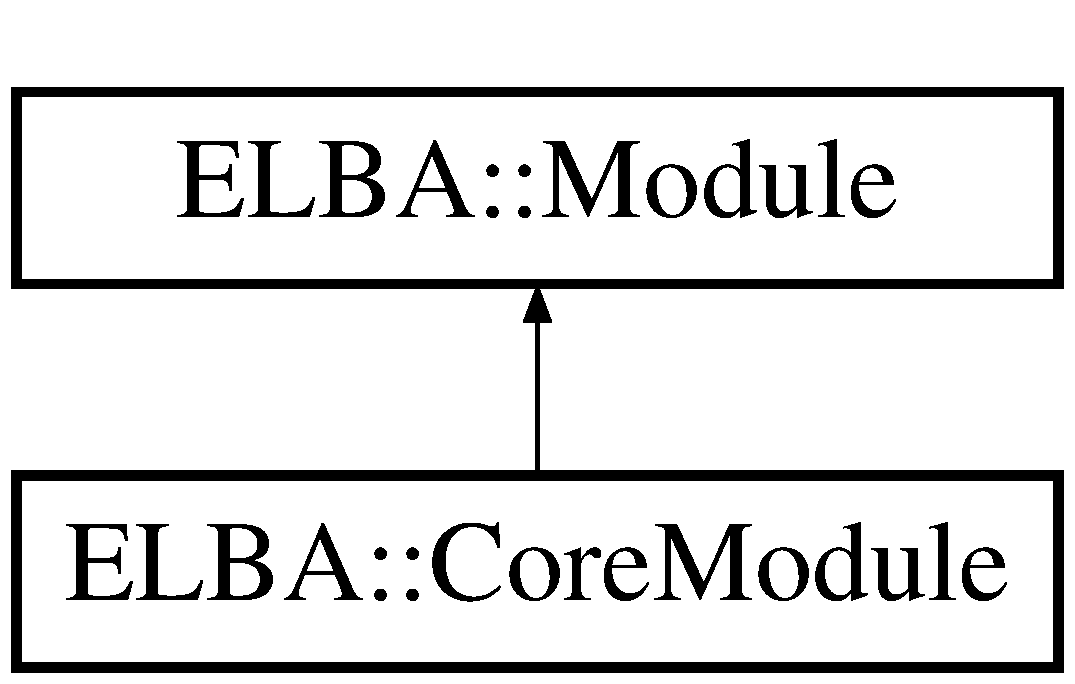
\includegraphics[height=2.000000cm]{class_e_l_b_a_1_1_core_module}
\end{center}
\end{figure}
\subsection*{Public Member Functions}
\begin{DoxyCompactItemize}
\item 
\mbox{\Hypertarget{class_e_l_b_a_1_1_core_module_a329d759e13e82905d86fc2586977064d}\label{class_e_l_b_a_1_1_core_module_a329d759e13e82905d86fc2586977064d}} 
\mbox{\hyperlink{class_e_l_b_a_1_1_core_module_a329d759e13e82905d86fc2586977064d}{Core\+Module}} ()
\begin{DoxyCompactList}\small\item\em constructor \end{DoxyCompactList}\item 
\mbox{\Hypertarget{class_e_l_b_a_1_1_core_module_a8a1cd3d0a6f1ae195187c45a3cfee744}\label{class_e_l_b_a_1_1_core_module_a8a1cd3d0a6f1ae195187c45a3cfee744}} 
void \mbox{\hyperlink{class_e_l_b_a_1_1_core_module_a8a1cd3d0a6f1ae195187c45a3cfee744}{Update}} () override
\begin{DoxyCompactList}\small\item\em Update function called by \mbox{\hyperlink{class_e_l_b_a_1_1_engine}{Engine}}. Updates all game objects. \end{DoxyCompactList}\end{DoxyCompactItemize}


\subsection{Detailed Description}
\mbox{\hyperlink{class_e_l_b_a_1_1_module}{Module}} for the core of the engine. Manages objects. 

The documentation for this class was generated from the following files\+:\begin{DoxyCompactItemize}
\item 
elba/\+Source/\+Core/\mbox{\hyperlink{_core_module_8hpp}{Core\+Module.\+hpp}}\item 
elba/\+Source/\+Core/\mbox{\hyperlink{_core_module_8cpp}{Core\+Module.\+cpp}}\end{DoxyCompactItemize}

\hypertarget{class_e_l_b_a_1_1_engine}{}\section{E\+L\+BA\+:\+:Engine Class Reference}
\label{class_e_l_b_a_1_1_engine}\index{E\+L\+B\+A\+::\+Engine@{E\+L\+B\+A\+::\+Engine}}


Handles all the modules that comprise the game engine.  




{\ttfamily \#include $<$Engine.\+hpp$>$}

\subsection*{Public Member Functions}
\begin{DoxyCompactItemize}
\item 
\mbox{\Hypertarget{class_e_l_b_a_1_1_engine_a9f205a0bef747c264ac44d9185ffdbf8}\label{class_e_l_b_a_1_1_engine_a9f205a0bef747c264ac44d9185ffdbf8}} 
\mbox{\hyperlink{class_e_l_b_a_1_1_engine_a9f205a0bef747c264ac44d9185ffdbf8}{Engine}} ()
\begin{DoxyCompactList}\small\item\em cstor \end{DoxyCompactList}\end{DoxyCompactItemize}


\subsection{Detailed Description}
Handles all the modules that comprise the game engine. 

The documentation for this class was generated from the following file\+:\begin{DoxyCompactItemize}
\item 
elba/\+Source/\mbox{\hyperlink{_engine_8hpp}{Engine.\+hpp}}\end{DoxyCompactItemize}

\hypertarget{class_e_l_b_a_1_1_graphics_module}{}\section{E\+L\+BA\+:\+:Graphics\+Module Class Reference}
\label{class_e_l_b_a_1_1_graphics_module}\index{E\+L\+B\+A\+::\+Graphics\+Module@{E\+L\+B\+A\+::\+Graphics\+Module}}


\mbox{\hyperlink{class_e_l_b_a_1_1_module}{Module}} for the graphics system. Manages rendering.  




{\ttfamily \#include $<$Graphics\+Module.\+hpp$>$}

Inheritance diagram for E\+L\+BA\+:\+:Graphics\+Module\+:\begin{figure}[H]
\begin{center}
\leavevmode
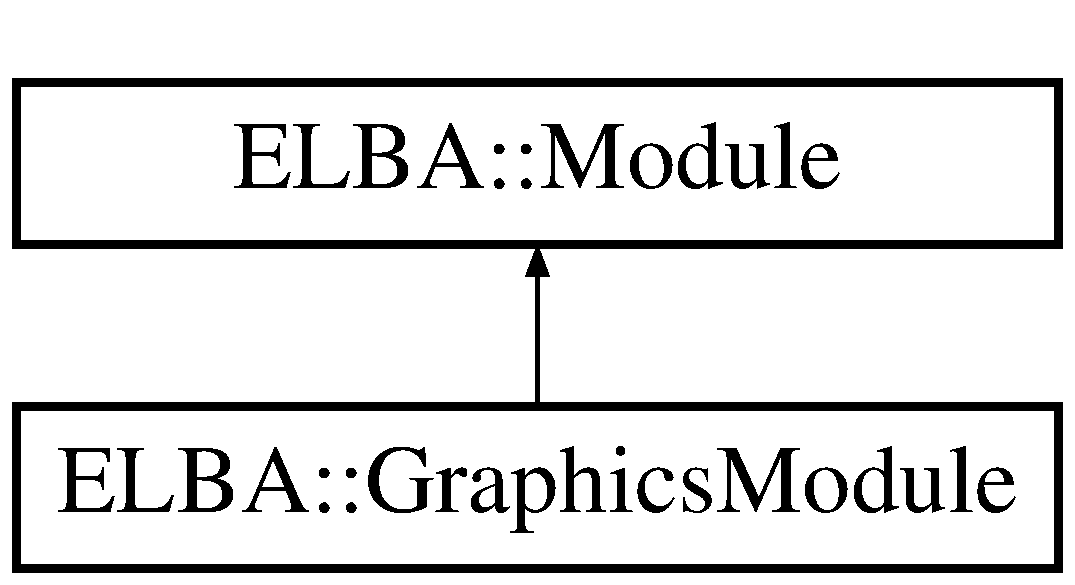
\includegraphics[height=2.000000cm]{class_e_l_b_a_1_1_graphics_module}
\end{center}
\end{figure}
\subsection*{Public Member Functions}
\begin{DoxyCompactItemize}
\item 
\mbox{\Hypertarget{class_e_l_b_a_1_1_graphics_module_ab9a67cab79cbdbd2b53c51955d6f137c}\label{class_e_l_b_a_1_1_graphics_module_ab9a67cab79cbdbd2b53c51955d6f137c}} 
\mbox{\hyperlink{class_e_l_b_a_1_1_graphics_module_ab9a67cab79cbdbd2b53c51955d6f137c}{Graphics\+Module}} ()
\begin{DoxyCompactList}\small\item\em cstor \end{DoxyCompactList}\item 
\mbox{\Hypertarget{class_e_l_b_a_1_1_graphics_module_a610a0dcdef572635b06de3a8a01d3375}\label{class_e_l_b_a_1_1_graphics_module_a610a0dcdef572635b06de3a8a01d3375}} 
void \mbox{\hyperlink{class_e_l_b_a_1_1_graphics_module_a610a0dcdef572635b06de3a8a01d3375}{Update}} () override
\begin{DoxyCompactList}\small\item\em Update function called by \mbox{\hyperlink{class_e_l_b_a_1_1_engine}{Engine}}. Updates graphics. \end{DoxyCompactList}\end{DoxyCompactItemize}


\subsection{Detailed Description}
\mbox{\hyperlink{class_e_l_b_a_1_1_module}{Module}} for the graphics system. Manages rendering. 

The documentation for this class was generated from the following files\+:\begin{DoxyCompactItemize}
\item 
elba/\+Source/\+Graphics/\mbox{\hyperlink{_graphics_module_8hpp}{Graphics\+Module.\+hpp}}\item 
elba/\+Source/\+Graphics/\mbox{\hyperlink{_graphics_module_8cpp}{Graphics\+Module.\+cpp}}\end{DoxyCompactItemize}

\hypertarget{class_e_l_b_a_1_1_module}{}\section{E\+L\+BA\+:\+:Module Class Reference}
\label{class_e_l_b_a_1_1_module}\index{E\+L\+B\+A\+::\+Module@{E\+L\+B\+A\+::\+Module}}


Base class for systems that comprise the engine.  




{\ttfamily \#include $<$Module.\+hpp$>$}

Inheritance diagram for E\+L\+BA\+:\+:Module\+:\begin{figure}[H]
\begin{center}
\leavevmode
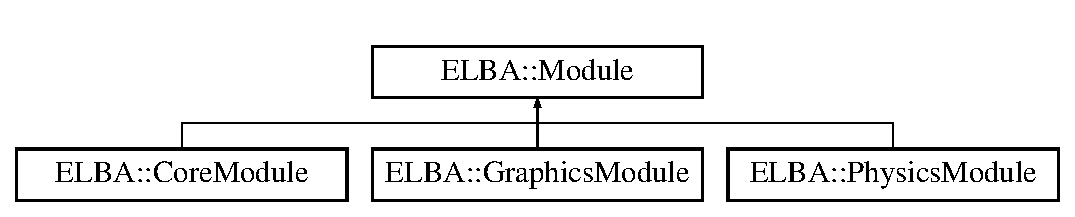
\includegraphics[height=2.000000cm]{class_e_l_b_a_1_1_module}
\end{center}
\end{figure}
\subsection*{Public Member Functions}
\begin{DoxyCompactItemize}
\item 
\mbox{\Hypertarget{class_e_l_b_a_1_1_module_af35ca6b0cec41f471adff4145767927c}\label{class_e_l_b_a_1_1_module_af35ca6b0cec41f471adff4145767927c}} 
\mbox{\hyperlink{class_e_l_b_a_1_1_module_af35ca6b0cec41f471adff4145767927c}{Module}} ()
\begin{DoxyCompactList}\small\item\em cstor \end{DoxyCompactList}\item 
\mbox{\Hypertarget{class_e_l_b_a_1_1_module_a9f7461e29016c9b246c9888fe5534b85}\label{class_e_l_b_a_1_1_module_a9f7461e29016c9b246c9888fe5534b85}} 
virtual void \mbox{\hyperlink{class_e_l_b_a_1_1_module_a9f7461e29016c9b246c9888fe5534b85}{Update}} ()=0
\begin{DoxyCompactList}\small\item\em Update function that \mbox{\hyperlink{class_e_l_b_a_1_1_engine}{Engine}} will call on each module. \end{DoxyCompactList}\end{DoxyCompactItemize}


\subsection{Detailed Description}
Base class for systems that comprise the engine. 

The documentation for this class was generated from the following files\+:\begin{DoxyCompactItemize}
\item 
elba/\+Source/\+Framework/\mbox{\hyperlink{_module_8hpp}{Module.\+hpp}}\item 
elba/\+Source/\+Framework/\mbox{\hyperlink{_module_8cpp}{Module.\+cpp}}\end{DoxyCompactItemize}

\hypertarget{class_e_l_b_a_1_1_object}{}\section{E\+L\+BA\+:\+:Object Class Reference}
\label{class_e_l_b_a_1_1_object}\index{E\+L\+B\+A\+::\+Object@{E\+L\+B\+A\+::\+Object}}


Any possible object in the game.  




{\ttfamily \#include $<$Object.\+hpp$>$}

\subsection*{Public Member Functions}
\begin{DoxyCompactItemize}
\item 
\mbox{\Hypertarget{class_e_l_b_a_1_1_object_aa3abbb9687693d254ada1d0b6573c40e}\label{class_e_l_b_a_1_1_object_aa3abbb9687693d254ada1d0b6573c40e}} 
\mbox{\hyperlink{class_e_l_b_a_1_1_object_aa3abbb9687693d254ada1d0b6573c40e}{Object}} ()
\begin{DoxyCompactList}\small\item\em cstor \end{DoxyCompactList}\end{DoxyCompactItemize}


\subsection{Detailed Description}
Any possible object in the game. 

The documentation for this class was generated from the following files\+:\begin{DoxyCompactItemize}
\item 
elba/\+Source/\+Core/\mbox{\hyperlink{_object_8hpp}{Object.\+hpp}}\item 
elba/\+Source/\+Core/\mbox{\hyperlink{_object_8cpp}{Object.\+cpp}}\end{DoxyCompactItemize}

\chapter{File Documentation}
\hypertarget{_core_module_8hpp}{}\section{elba/\+Source/\+Core/\+Core\+Module.hpp File Reference}
\label{_core_module_8hpp}\index{elba/\+Source/\+Core/\+Core\+Module.\+hpp@{elba/\+Source/\+Core/\+Core\+Module.\+hpp}}


Class definition for Core\+Module.  


{\ttfamily \#include \char`\"{}Framework/\+Module.\+hpp\char`\"{}}\newline
\subsection*{Classes}
\begin{DoxyCompactItemize}
\item 
class \mbox{\hyperlink{class_e_l_b_a_1_1_core_module}{E\+L\+B\+A\+::\+Core\+Module}}
\begin{DoxyCompactList}\small\item\em \mbox{\hyperlink{class_e_l_b_a_1_1_module}{Module}} for the core of the engine. Manages objects. \end{DoxyCompactList}\end{DoxyCompactItemize}


\subsection{Detailed Description}
Class definition for Core\+Module. 

\begin{DoxyAuthor}{Author}
Nicholas Ammann 
\end{DoxyAuthor}
\begin{DoxyDate}{Date}
2/24/2018 
\end{DoxyDate}

\hypertarget{_object_8hpp}{}\section{elba/\+Source/\+Core/\+Object.hpp File Reference}
\label{_object_8hpp}\index{elba/\+Source/\+Core/\+Object.\+hpp@{elba/\+Source/\+Core/\+Object.\+hpp}}


Class definition for Object.  


\subsection*{Classes}
\begin{DoxyCompactItemize}
\item 
class \mbox{\hyperlink{class_e_l_b_a_1_1_object}{E\+L\+B\+A\+::\+Object}}
\begin{DoxyCompactList}\small\item\em Any possible object in the game. \end{DoxyCompactList}\end{DoxyCompactItemize}


\subsection{Detailed Description}
Class definition for Object. 

\begin{DoxyAuthor}{Author}
Nicholas Ammann 
\end{DoxyAuthor}
\begin{DoxyDate}{Date}
2/24/2018 
\end{DoxyDate}

\hypertarget{_engine_8hpp}{}\section{elba/\+Source/\+Engine.hpp File Reference}
\label{_engine_8hpp}\index{elba/\+Source/\+Engine.\+hpp@{elba/\+Source/\+Engine.\+hpp}}


Class definition for Engine.  


{\ttfamily \#include \char`\"{}Core/\+Core\+Forward\+Declarations.\+hpp\char`\"{}}\newline
{\ttfamily \#include \char`\"{}Graphics/\+Graphics\+Forward\+Declarations.\+hpp\char`\"{}}\newline
{\ttfamily \#include \char`\"{}Physics/\+Physics\+Forward\+Declarations.\+hpp\char`\"{}}\newline
\subsection*{Classes}
\begin{DoxyCompactItemize}
\item 
class \mbox{\hyperlink{class_e_l_b_a_1_1_engine}{E\+L\+B\+A\+::\+Engine}}
\begin{DoxyCompactList}\small\item\em Handles all the modules that comprise the game engine. \end{DoxyCompactList}\end{DoxyCompactItemize}


\subsection{Detailed Description}
Class definition for Engine. 

\begin{DoxyAuthor}{Author}
Nicholas Ammann 
\end{DoxyAuthor}
\begin{DoxyDate}{Date}
2/24/2018 
\end{DoxyDate}

\hypertarget{_module_8hpp}{}\section{elba/\+Source/\+Framework/\+Module.hpp File Reference}
\label{_module_8hpp}\index{elba/\+Source/\+Framework/\+Module.\+hpp@{elba/\+Source/\+Framework/\+Module.\+hpp}}


Class definition for Module.  


\subsection*{Classes}
\begin{DoxyCompactItemize}
\item 
class \mbox{\hyperlink{class_e_l_b_a_1_1_module}{E\+L\+B\+A\+::\+Module}}
\begin{DoxyCompactList}\small\item\em Base class for systems that comprise the engine. \end{DoxyCompactList}\end{DoxyCompactItemize}


\subsection{Detailed Description}
Class definition for Module. 

\begin{DoxyAuthor}{Author}
Nicholas Ammann 
\end{DoxyAuthor}
\begin{DoxyDate}{Date}
2/24/2018 
\end{DoxyDate}

\hypertarget{_graphics_module_8hpp}{}\section{elba/\+Source/\+Graphics/\+Graphics\+Module.hpp File Reference}
\label{_graphics_module_8hpp}\index{elba/\+Source/\+Graphics/\+Graphics\+Module.\+hpp@{elba/\+Source/\+Graphics/\+Graphics\+Module.\+hpp}}


Class definition for Graphics\+Module.  


{\ttfamily \#include \char`\"{}Framework/\+Module.\+hpp\char`\"{}}\newline
\subsection*{Classes}
\begin{DoxyCompactItemize}
\item 
class \mbox{\hyperlink{class_e_l_b_a_1_1_graphics_module}{E\+L\+B\+A\+::\+Graphics\+Module}}
\begin{DoxyCompactList}\small\item\em \mbox{\hyperlink{class_e_l_b_a_1_1_module}{Module}} for the graphics system. Manages rendering. \end{DoxyCompactList}\end{DoxyCompactItemize}


\subsection{Detailed Description}
Class definition for Graphics\+Module. 

\begin{DoxyAuthor}{Author}
Nicholas Ammann 
\end{DoxyAuthor}
\begin{DoxyDate}{Date}
2/24/2018 
\end{DoxyDate}

%--- End generated contents ---

% Index
\backmatter
\newpage
\phantomsection
\clearemptydoublepage
\addcontentsline{toc}{chapter}{Index}
\printindex

\end{document}
